\appendix
%\chapter{Proof of Theorem 1}\label{appendix1}
\chapter{パラメータ候補の比較}\label{ch:appendix}
\begin{figure}[H]
  \begin{center}
    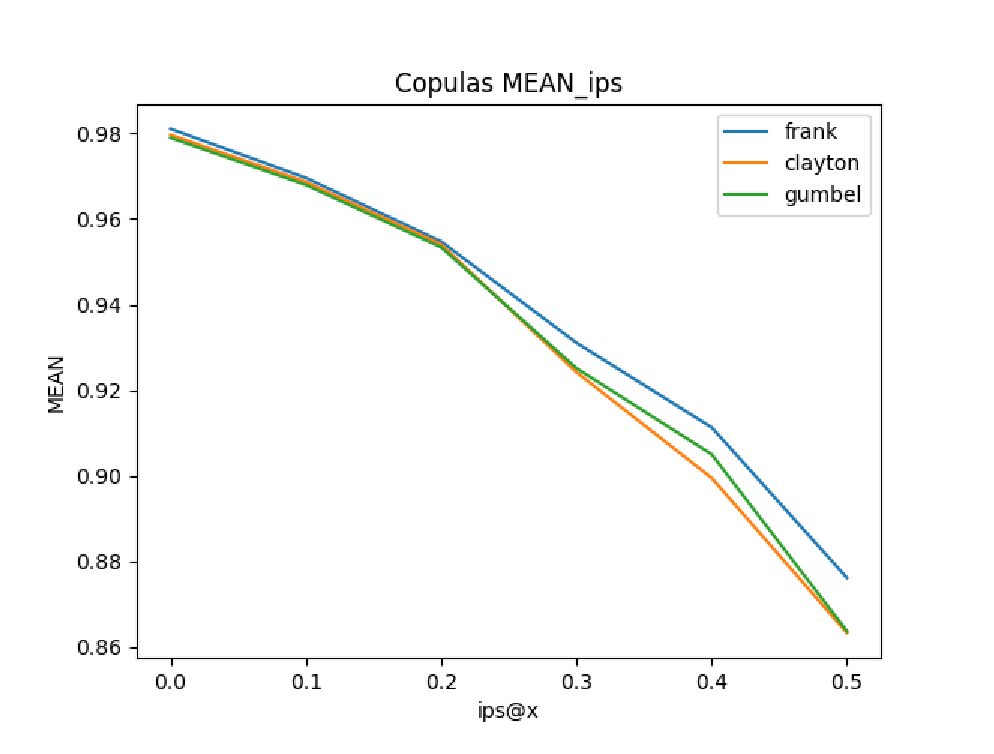
\includegraphics[width=7in]{source/copula_ip.eps}
  \vspace{1mm}
  \caption{コピュラのiP比較} %\vspace{-3mm}
  \label{fig:copula_ip}
  %\vspace{-0.4cm}
  \end{center} 
\end{figure}
\begin{figure}[H]
  \begin{center}
    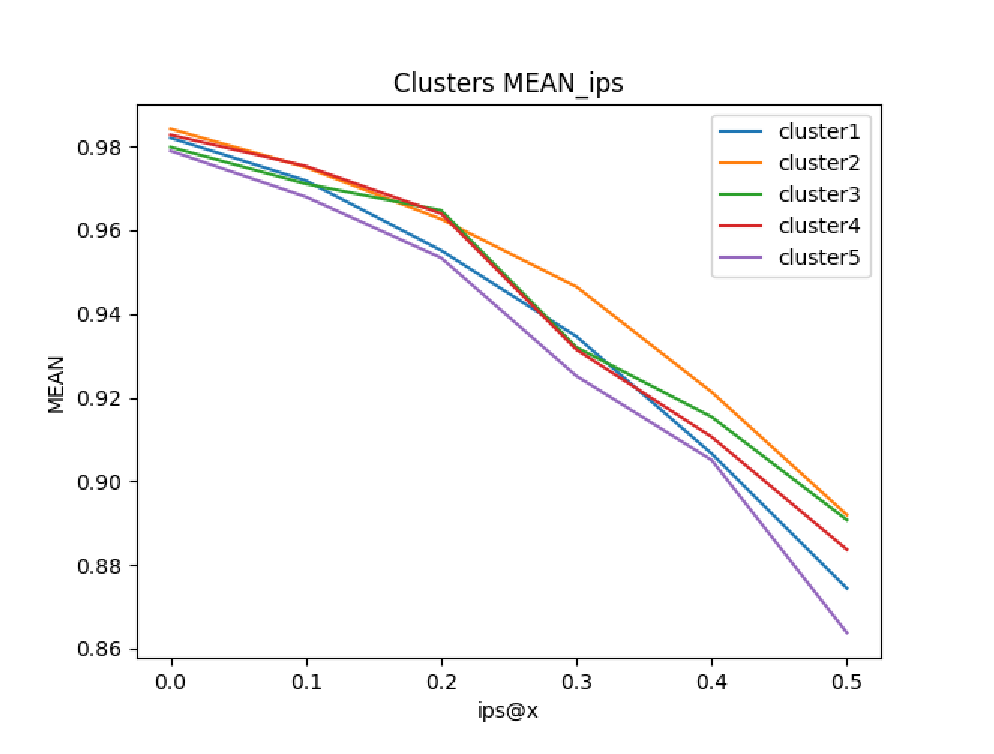
\includegraphics[width=7in]{source/cluster_ip.eps}
  \vspace{1mm}
  \caption{クラスタ数のiP比較} %\vspace{-3mm}
  \label{fig:cluster_ip}
  %\vspace{-0.4cm}
  \end{center} 
\end{figure}
\begin{figure}[H]
  \begin{center}
    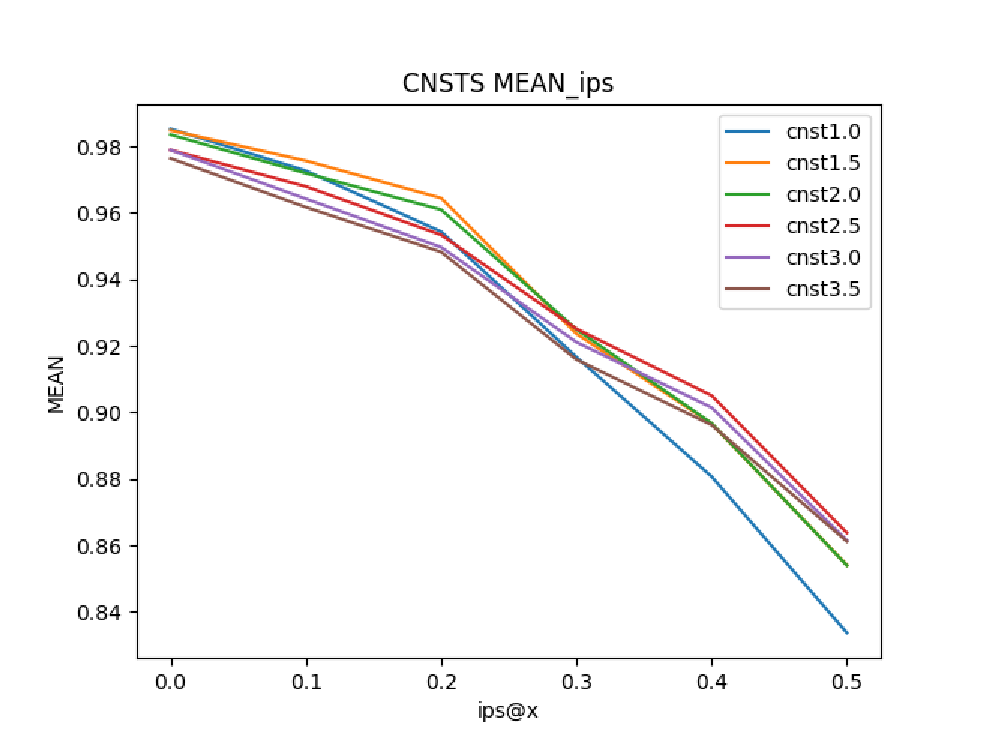
\includegraphics[width=7in]{source/cnst_ip.eps}
  \vspace{1mm}
  \caption{正定数cnstのiP比較} %\vspace{-3mm}
  \label{fig:cnst_ip}
  %\vspace{-0.4cm}
  \end{center} 
\end{figure}

%\chapter{Proof of Theorem 2}\label{appendix2}
%\chapter{定理2の証明}\label{appendix2}
